The implemented RL approach was able to successfully map the computation graphs for vector addition and multiply-add operations. 
Fig. 3 shows the increase in the value of the rewards obtained as the number of training iterations increase. 
As the reward increases, we obtain mappings with lesser total execution times. 

This method also presents an advantage compared to baselines random search and evolutionary search (ES) methods which do not learn. 
The RL approach can also learn from a collection of computation graphs and reuse the learning for mapping previously unseen computation graphs. 
The other methods on the other hand will have to perform a new search and start from scratch for every new computation graph. 
PPO with graph embeddings showed that we can obtain more optimized placements by finding higher rewards than other RL approaches. 

\begin{figure}[h]
    \centering
    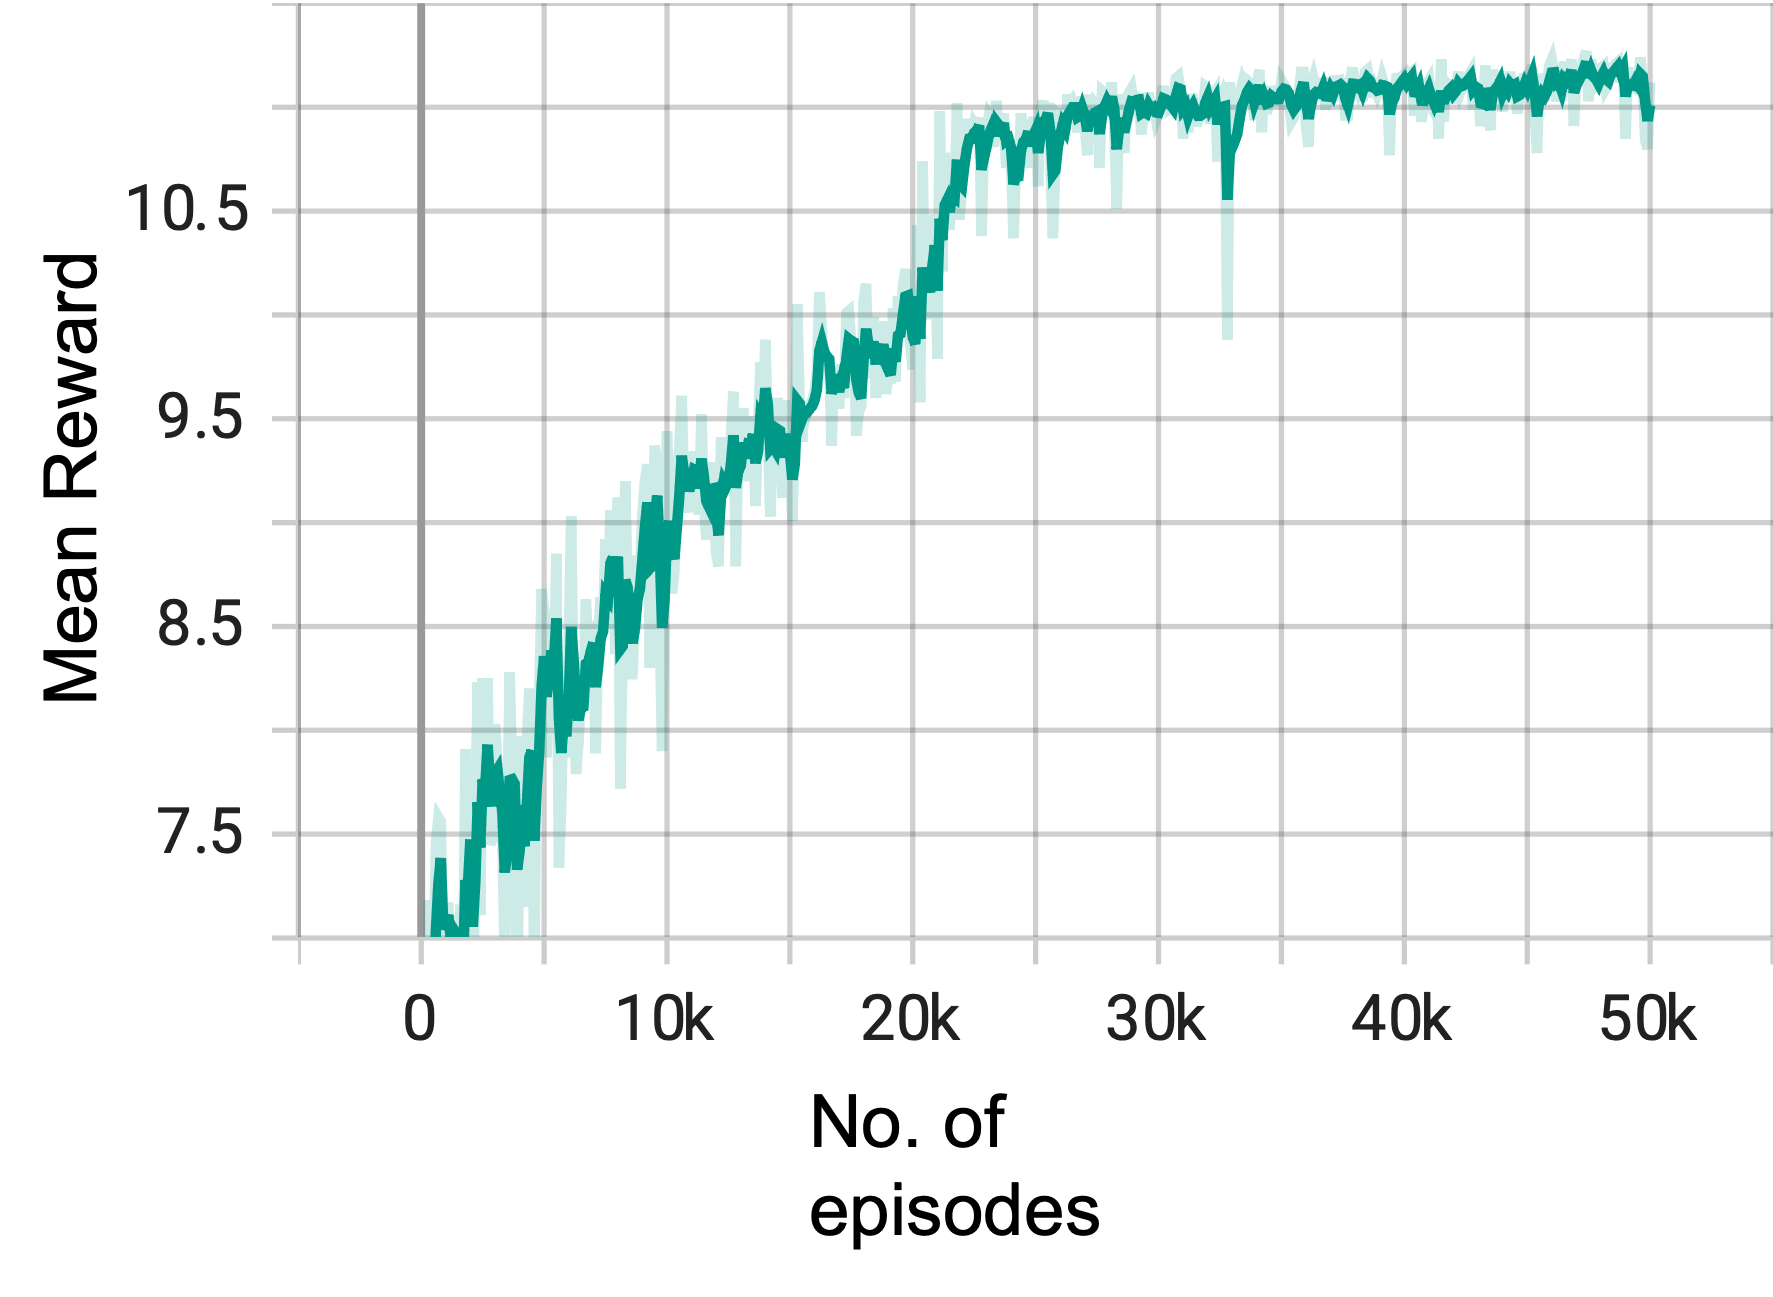
\includegraphics[width=\linewidth]{fig/ifft_rewards.png}
    \caption{Mean reward during training on ifft graph}
    \label{fig:ifft_rewards}
  \end{figure}

  \begin{figure}[h]
    \centering
    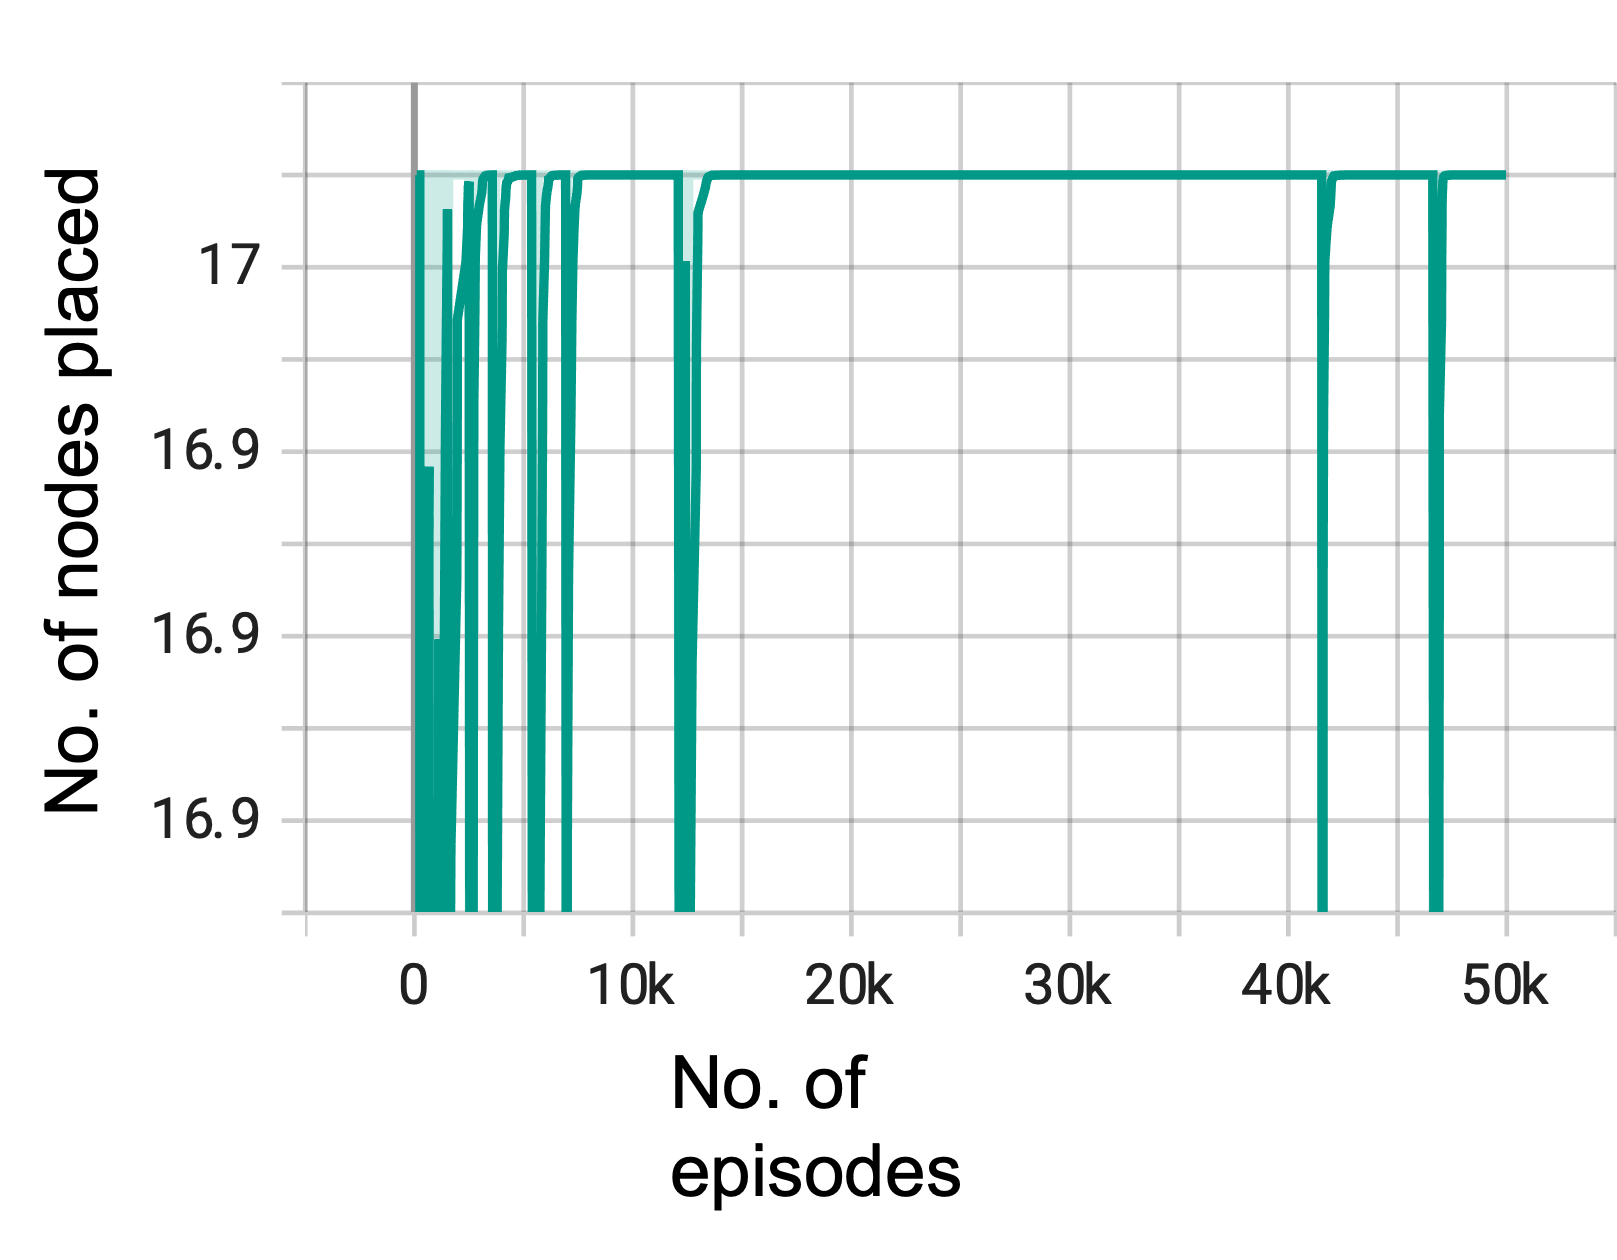
\includegraphics[width=\linewidth]{fig/ifft_nodes_placed.png}
    \caption{Number of ifft nodes placed per episode}
    \label{fig:ifft_rewards}
  \end{figure}

\subsection{Experimental Setup}

\subsection{Ablation study}